\documentclass[degree=tsxlx,bibtype=numeric,degreetype=kczy]{tongjithesis}

\setlength{\footskip}{15.61334pt}

% 其它可能用到的包
\usepackage{tongjiutils}

%参考文献更新使用biblatex包
\addbibresource{ref/refs.bib}   

\begin{document}

% 定义所有的eps文件在 figures 子目录下
\graphicspath{{figures/}}

% 封面
\frontmatter
\tongjisetup{
  %=========
  % 中文信息
  %=========
  ctitle={基于一种细长圆杆的多维弹塑性分析},
  cheadingtitle={基于一种细长圆杆的多维弹塑性分析},   
  cauthor={唐霖辉},  
  studentnumber={2410486},
  ccategories={工学},
  cmajorfirst={土木工程},
  cmajorsecond={结构工程},
  cdepartment={土木工程学院},
  csupervisor={何敏娟 教授}, 
  cresearchfield={大跨木结构},
  cassosupervisor={任晓丹 教授},
  %=========
  % 英文信息
  %=========
  etitle={Multi-dimensional elastoplastic analysis based on an elongated round rod}, 
  eauthor={Linhui Tang},
  ecategories={Gong Xue},
  emajorfirst={Civil Engineering},
  emajorsecond={Structural Engineering},
  edepartment={School of Civil Engineering},    
  esupervisor={Prof. Minjuan He},
  eassosupervisor={Prof. Xiaodan Ren},
  eresearchfield={Large-span timber construction},
  }
  %=========
  % 中英文摘要和关键字
  %=========
\begin{cabstract}  
  弹
\end{cabstract}

\ckeywords{弹塑性力学, 多维弹塑性理论, 屈服函数, 有限元分析}

\begin{eabstract}
  T.
\end{eabstract}

\ekeywords{elastoplasticity, multidimensional elastoplasticity theory, yield function, finite element analysis}
\makecover

% 目录
\tableofcontents

% 正文 
\mainmatter
\chapter{问题描述}
\label{cha:Description}
本章节对研究问题进行阐述,该问题选自《工程弹塑性力学引论》课本第七章课后习题\cite{gctsxyl}。本文将对该问题中的~6~个小题进行回答。

给定一根圆形截面细杆,已知: 

1.~长度为~{$L$},半径为~{$R$}; 

2.~构成材料为理想弹塑性材料,弹性模量~{$E$},泊松比~{$\nu$},屈服强度为~{$f_y$},服从~Mises~屈服准则。 

加载方式如下: 

1.~首先轴向拉伸细杆,使其全长全截面轴向应力均达到~{$f_y$}; 

2.~然后在保持杆长不变的情况下,杆的两个端截面相对旋转一个小角度~{$\theta$},假定扭转变形沿着杆的轴向均匀分布,同时杆的任意横截面在旋转过程中均保持平面。 

问:
 
1.~如何不经过计算,即判断杆的轴向应力在旋转变形过程中是变大还是变小? 

2.~推导上述变形之后,轴向应力与剪应力沿杆截面分布的解析表达式。

3.~其他条件不变,将材料考虑为各向同性线性硬化材料,硬化模量为~{$K$},推导上述问题的控制方程,并讨论此时是否可以得到问题的解析解。

4.~自拟一组参数(建议采用钢材的材料参数,钢材强度等级自定),进行上述问题的有限元分析(软件不限),比较理论结果与计算结果,讨论二者的区别与联系。 

5.~其他条件不变,将材料考虑为各向同性线性硬化材料,硬化模量取为~{$K=0.05E$},再进行有限元分析,根据计算结果讨论理想弹塑性材料与弹塑性硬化材料的区别。 

6.~如果改为~Drucker-Prager~塑性模型,结果将会怎样?
\chapter{简支梁平面问题的解析解}
\setlength{\footskip}{15.61334pt}
\label{cha:Analyticalsolution}
本章节主要讨论《工程弹塑性力学引论》例~B.2~中简支梁平面问题\cite{gctsxyl}的解析解,通过半逆解法来求解简支梁的应力、应变、位移场量,并对结果进行分析和可视化。
\section{平面问题描述}
所求解的简支梁如图\ref{fig:load}所示,长度为~$l$,截面宽度为单位~1,截面高度为~$h$。梁的上边缘受均布荷载~$q$~作用。在梁的质心处建立直角坐标系,沿长度方向为~$x$~轴,沿高度方向为~$y$~轴。考虑到该简支梁的截面高度远大于宽度,在求解时可以认为该问题是平面应力问题,因此解析解与~$z$~方向无关。
\begin{figure}[htbp]
    \centering
	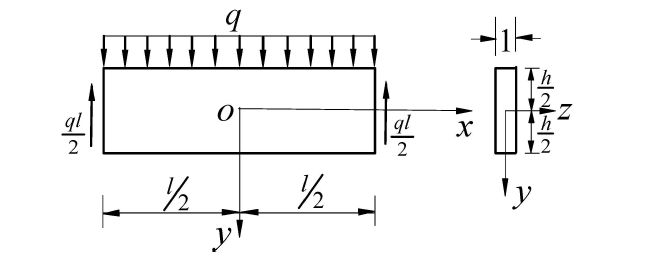
\includegraphics[width=0.7\textwidth]{figure1}
    \caption{简支梁承受均布荷载}
    \label{fig:load}
\end{figure}
\section{半逆解法求解}
\subsection{公式推导}
弹性力学的平面问题可以归结为以下三组方程:\\
1)平衡方程
\begin{equation}\label{eq1}
    \left\{
        \begin{array}{l}
            \dfrac{\partial \sigma_x}{\partial x} + \dfrac{\partial \tau_{xy}}{\partial y} + f_x = 0\\
            \dfrac{\partial \tau_{yx}}{\partial x} + \dfrac{\partial \sigma_y}{\partial y} + f_y = 0
        \end{array}
    \right.
\end{equation} 
2)协调方程
\begin{equation}\label{eq2}
    \frac{\partial^2 \varepsilon_x}{\partial x^2} +\frac{\partial^2 \varepsilon_y}{\partial y^2} = 2\frac{\partial^2 \varepsilon_{xy}}{\partial x \partial y}
\end{equation} 
3)应力-应变关系
\begin{equation}\label{eq3}
    \left\{
        \begin{array}{l}
            \varepsilon_x = \dfrac{1}{E}(\sigma_x-\nu \sigma_y)\vspace{1ex}\\
            \varepsilon_y = \dfrac{1}{E}(\sigma_y-\nu \sigma_x)\vspace{1ex}\\
            \varepsilon_{xy} = \dfrac{1}{2G}\tau_{xy}
        \end{array}
    \right.
\end{equation} 

将应力-应变关系\eqref{eq3}和平衡方程\eqref{eq1}代入协调方程\eqref{eq2},且不考虑体力,可化简得到:
\begin{equation}\label{eq4}
    \bigtriangledown^2(\sigma_x+\sigma_y) = 0
\end{equation} 

再考虑无体力的平衡方程:
\begin{equation}\label{eq5}
    \left\{
        \begin{array}{l}
            \dfrac{\partial \sigma_x}{\partial x} + \dfrac{\partial \tau_{xy}}{\partial y} = 0\vspace{1ex}\\
            \dfrac{\partial \tau_{yx}}{\partial x} + \dfrac{\partial \sigma_y}{\partial y} = 0
        \end{array}
    \right.
\end{equation} 
结合格林(Green)定理,可知存在势函数~$P$~和~$Q$,满足:
\begin{equation}\label{eq6}
    \sigma_x = \frac{\partial P}{\partial y}~,~\tau_{xy} = -\frac{\partial P}{\partial x}~,~\sigma_y = \frac{\partial Q}{\partial x}~,~\tau_{yx} = -\frac{\partial Q}{\partial y}
\end{equation}  

进一步结合剪应力互等定理,剪力满足:
\begin{equation}\label{eq7}
    \tau_{xy}-\tau_{yx} = \frac{\partial Q}{\partial y}-\frac{\partial P}{\partial x}=0
\end{equation}  
同样可以使用格林定理得到势函数~$\phi$,满足:
\begin{equation}\label{eq8}
    P = \frac{\partial \phi}{\partial y}~,~Q = \frac{\partial \phi}{\partial x}
\end{equation}  
其中~$\phi$~为艾里(Airy)应力函数。将~$P$、~$Q$~代入式\eqref{eq6},可得应力分量方程:
\begin{equation}\label{eq9}
    \sigma_x = \frac{\partial^2 \phi}{\partial y^2}~,~\sigma_y = \frac{\partial^2 \phi}{\partial x^2}~,~\tau_{xy} = -\frac{\partial^2 \phi}{\partial x \partial y}
\end{equation} 
再将\eqref{eq9}带入简化后的无体力协调方程\eqref{eq4},整理可得应力函数方程:
\begin{equation}\label{eq10}
    \bigtriangledown^2\bigtriangledown^2 \phi = 0
\end{equation}
其中~$\bigtriangledown^2\bigtriangledown^2$~被称为双调和算符。

在半逆解法中,应力函数的构成可以考虑微分方程解法中的分离变量法,假定应力函数的形式为:
\begin{equation}\label{eq11}
    \phi = g(x)f(y)
\end{equation}
带入双调和方程\eqref{eq10},有:
\begin{equation}\label{eq12}
    \bigtriangledown^2\bigtriangledown^2 \phi = g''''(x)f(y)+2g''(x)f''(y)+g(x)f''''(y) = 0
\end{equation}
若考虑函数~$g(x)$~为多项式形式,将多项式带入式\eqref{eq12},可得关于~$f(y)$、$f^{''}(y)$、$f^{''''}(y)$~构成系数的多项式方程。该方程恒等于~0~的条件是系数恒等于0。由此可建立~$f(y)$~的微分方程,进而求出~$f(y)$~的表达式。若应力函数是\eqref{eq11}的线性组合,即:
\begin{equation}\label{eq13}
    \phi = \sum_{i} g_i(x)f_i(y)
\end{equation}
仍可以用上述过程求解。
\subsection{问题求解}
首先对问题进行简单的分析,$\sigma_x$~主要是由弯矩引起,$\sigma_y$~主要是由~$q$~引起(挤压应力),$\tau_{xy}$~主要是由剪力引起。又因为~$q$~恒定不变,且结构在图示坐标系下对称,因此假定~$\sigma_y$~与~$x$~无关,推得:
\begin{equation}\label{eq14}
    \sigma_y = \frac{\partial^2 \phi}{\partial x^2} = f(y)
\end{equation}
对上式积分,可得应力函数~$\phi$~的基本表达式为:
\begin{equation}\label{eq15}
    \phi = \frac{1}{2}x^2f(y)+xf_1(y)+f_2(y)
\end{equation}
其中~$f(y)$、~$f_1(y)$、$f_2(y)$~为任意待定的多项式函数。
进一步通过式\eqref{eq9}求得其中~$\tau_{xy}$~的表达式为:
\begin{equation}\label{eq16}
    \tau_{xy} = -\frac{\partial^2 \phi}{\partial x \partial y} = -xf'(y)+f_1'(y)
\end{equation}

接着观察到剪应力~$\tau_{xy}$~关于~y~轴反对称,是关于~x~的奇函数,因此上式中的~$f_1'(y)$~恒等于~0,从而推得:
\begin{equation}\label{eq17}
    \tau_{xy} = -xf'(y)
\end{equation}
对~$\tau_{xy}$~积分,反推得应力函数~$\phi$~修正表达式为:
\begin{equation}\label{eq18}
    \phi = \frac{1}{2}x^2f(y)+f_2(y)
\end{equation}  

将修正的表达式代入式\eqref{eq12},可得:
\begin{equation}\label{eq19}
    \frac{1}{2}x^2f''''(y)+ 2f''(y)+f_2''''(y) = 0
\end{equation}  
该关于x的系数方程恒成立的条件为系数恒等于~0,即:
\begin{equation}\label{eq20}
    \left\{
        \begin{array}{l}
            \dfrac{1}{2}f''''(y) = 0 \\
            2f''(y)+f_2''''(y) = 0
        \end{array}
    \right.
\end{equation} 
利用多次不定积分,可得上述微分方程组的解如下:
\begin{equation}\label{eq21}
    \left\{
        \begin{array}{l}
            f(y) = \text{A}+\text{B}y+\text{C}y^2+\text{D}y^3 \\
            f_2(y) = \text{E}+\text{F}y+\text{G}y^2+\text{H}y^3-\dfrac{1}{6}\text{C}y^4-\dfrac{1}{10}\text{D}y^5
        \end{array}
    \right.
\end{equation}
其中,A$\sim$H~均为待定系数;将上式代入式\eqref{eq18}后,再将得出的~$\phi$~回代入式\eqref{eq9},可得应力函数的表达式为:
\begin{equation}\label{eq22}
    \left\{
        \begin{array}{l}
            \sigma_x = \dfrac{1}{2}x^2f''(y)+f''_2(y) = \dfrac{1}{2}x^2(2\text{C}+6\text{D}y)+2\text{G}+6\text{H}y-2\text{C}y^3-2\text{D}y^4\\
            \sigma_y = f(y) = \text{A}+\text{B}y+\text{C}y^2+\text{D}y^3\\
            \tau_{xy} = -xf'(y) = -x(\text{B}+2\text{C}y+3\text{D}y^2)
        \end{array}
    \right.
\end{equation}

为了求解应力函数中的待定系数,需要利用该问题的边界条件。对于基于应力求解,用位移边界条件还需积分,较难处理,故一般都化为力边界条件代入。上下两个边界为主要边界,应该严格满足边界条件,左右两个次要边界可以用圣维南原理不严格满足,其中:\\
1)主要边界条件(上下两侧的应力)
\begin{subequations}\label{eq23}
    \begin{numcases} 
         ~~\sigma_y = 0, &\mbox{y = $\dfrac{1}{2}h$}\label{eq23a}  \\
         ~\sigma_y = -q, &\mbox{y = $-\dfrac{1}{2}h$}\label{eq23b} \\
         ~\tau_{xy} = 0, &\mbox{y = $\pm$ $\dfrac{1}{2}h$}\label{eq23c}
    \end{numcases}
\end{subequations}
2)次要边界条件(左右两端的轴力、剪力、弯矩)
\begin{subequations}\label{eq24} 
    \begin{numcases}  
         ~~\int_{-h/2}^{h/2}\sigma_x dy = 0, &\mbox{x = $\pm$ $\dfrac{1}{2}l$}\label{eq24a} \\
         ~\int_{-h/2}^{h/2}\tau_{xy} dy = -\frac{1}{2}ql, &\mbox{x = $\pm$ $\dfrac{1}{2}l$}\label{eq24b}\\
         ~\int_{-h/2}^{h/2}\sigma_xy dy = 0, &\mbox{x = $\pm$ $\dfrac{1}{2}l$}\label{eq24c}
    \end{numcases}
\end{subequations}
由式\eqref{eq23c}计算可得待定系数~C~=~0,B~=~$-\dfrac{3}{4}Dh^2$。将计算所得的系数值继续代入式\eqref{eq23a}和\eqref{eq23b},计算可得系数A~=~$-\dfrac{1}{2}q$,B~=~$\dfrac{3}{2h}q$,D~=~$-\dfrac{2}{h^3}q$。继续将已知的所有系数值代入式\eqref{eq24a}和\eqref{eq23c},计算可得系数G~=~0,H~=~$\dfrac{1}{4h^3}ql^2-\dfrac{1}{10h}q$。

将所求的全部系数值代入式\eqref{eq22},可得最终的应力函数表达式:
\begin{equation}\label{eq25}
    \left\{
        \begin{array}{l}
            \sigma_x = -\dfrac{6q}{h^3}x^2y+\dfrac{4q}{h^3}y^3+(\dfrac{3ql^2}{2h^3}-\dfrac{3q}{5h})y \vspace{1ex}\\
            \sigma_y = -\dfrac{2q}{h^3}y^3+\dfrac{3q}{2h}y-\dfrac{q}{2} \vspace{1ex}\\
            \tau_{xy} = \dfrac{6q}{h^3}xy^2-\dfrac{3q}{2h}x
        \end{array}
    \right.
\end{equation}  

将求解出的应力函数代入应力-应变关系式\eqref{eq3},可得应变函数表达式:
\begin{equation}\label{eq26}
    \left\{
        \begin{array}{l}
            \varepsilon_x = -\dfrac{6q}{Eh^3}x^2y+\dfrac{4q+2\nu q}{Eh^3}y^3+(\dfrac{3ql^2}{2Eh^3}-\dfrac{3q}{5Eh}-\dfrac{3\nu q}{2Eh})y+\dfrac{\nu q}{2E} \vspace{1ex}\\
            \varepsilon_y = \dfrac{6\nu q}{Eh^3}x^2y-\dfrac{4\nu q+2q}{Eh^3}y^3+(\dfrac{3q}{2Eh}+\dfrac{3\nu q}{5Eh}-\dfrac{3\nu ql^2}{2Eh^3})y-\dfrac{q}{2E} \vspace{1ex}\\
            \varepsilon_{xy} = \dfrac{6q}{2Gh^3}xy^2-\dfrac{3q}{4Gh}x
        \end{array}
    \right.
\end{equation}  

由位移和应变函数之间的微分关系:
\begin{subequations}\label{eq27}
    \begin{numcases}  
             ~~\varepsilon_x = \dfrac{\partial u}{\partial x}\vspace{1ex}\\
             ~\varepsilon_y = \dfrac{\partial v}{\partial y}\vspace{1ex}\\
             ~\varepsilon_{xy} = \dfrac{1}{2}(\dfrac{\partial u}{\partial y}+\dfrac{\partial v}{\partial x})\label{eq27c}
    \end{numcases}
\end{subequations}
可以推出位移函数表达式需满足:
\begin{equation}\label{eq28}
    \left\{
        \begin{array}{l}
            u = -\dfrac{2q}{Eh^3}x^3y+\dfrac{4q+2\nu q}{Eh^3}xy^3+(\dfrac{3ql^2}{2Eh^3}-\dfrac{3q}{5Eh}-\dfrac{3\nu q}{2Eh})xy+\dfrac{\nu q}{2E}x+f_3(y) \vspace{1ex}\\
            v = \dfrac{3\nu q}{Eh^3}x^2y^2-\dfrac{2\nu q+q}{2Eh^3}y^4+(\dfrac{3q}{4Eh}+\dfrac{3\nu q}{10Eh}-\dfrac{3\nu ql^2}{4Eh^3})y^2-\dfrac{q}{2E}y+f_4(x)
        \end{array}
    \right.
\end{equation}
其中~$f_3(y)$~和~$f_4(x)$~为待定多项式,将上式代入式\eqref{eq27c},化简得到~$f_3(y)$~和~$f_4(x)$~之间的关系需满足:
\begin{equation}\label{eq29}
    f'_3(y) = \dfrac{2q}{Eh^3}x^3-(\dfrac{3ql^2}{2Eh^3}+\dfrac{12q}{5Eh}+\dfrac{3\nu q}{2Eh})x-f'_4(x)
\end{equation}
观察式\eqref{eq29},发现等号左端仅为关于y的方程,等号右端仅为关于x的方程,若该式恒成立,则需满足:
\begin{equation}\label{eq30}
    f'_3(y) = \dfrac{2q}{Eh^3}x^3-(\dfrac{3ql^2}{2Eh^3}+\dfrac{12q}{5Eh}+\dfrac{3\nu q}{2Eh})x-f'_4(x)=\alpha_1
\end{equation}
其中~$\alpha_1$~为常数。此时通过积分,~$f_3(y)$~和~$f_4(x)$~的形式可以改写为:
\begin{equation}\label{eq31}
    \left\{
        \begin{array}{l}
            f_3(y) = \alpha_1y+\alpha_2 \\
            f_4(x) = \dfrac{q}{2Eh^3}x^4-(\dfrac{3ql^2}{4Eh^3}+\dfrac{6q}{5Eh}+\dfrac{3\nu q}{4Eh})x^2-\alpha_1x+\alpha_3
        \end{array}
    \right.
\end{equation}
\\其中~$\alpha_2$~和~$\alpha_3$~同样为常数。结合式\eqref{eq28}和式\eqref{eq31},可以得到含有待定系数的位移函数。为了求解位移函数中的待定系数,需要利用该问题的位移边界条件:
\begin{subequations}\label{eq32}
    \begin{numcases} 
         ~~u = 0, &\mbox{y= 0,~x = $-\dfrac{1}{2}l$} \vspace{1ex}\label{eq32a}  \\
         ~v = 0, &\mbox{y= 0,~x = $\pm \dfrac{1}{2}l$}\label{eq32b}
    \end{numcases}
\end{subequations}
由式\eqref{eq32a}计算可得待定系数~$\alpha_2$~=~$\dfrac{\nu ql}{4E}$,由式\eqref{eq32b}计算可得待定系数~$\alpha_3$~=~$\dfrac{5ql^4}{32Eh^3}+\dfrac{3ql^2}{10Eh}+\dfrac{3\nu ql^2}{16Eh}$,~$\alpha_1$~=~0。因此,最终的位移函数表达式为:
\begin{equation}\label{eq33}
    \left\{
        \begin{array}{l}
            u = -\dfrac{2q}{Eh^3}x^3y+\dfrac{4q+2\nu q}{Eh^3}xy^3+(\dfrac{3ql^2}{2Eh^3}-\dfrac{3q}{5Eh}-\dfrac{3\nu q}{2Eh})xy+\dfrac{\nu q}{2E}x+\dfrac{\nu ql}{4E} \vspace{1ex}\\
            v = \dfrac{3\nu q}{Eh^3}x^2y^2-\dfrac{2\nu q+q}{2Eh^3}y^4+(\dfrac{3q}{4Eh}+\dfrac{3\nu q}{10Eh}-\dfrac{3\nu ql^2}{4Eh^3})y^2-\dfrac{q}{2E}y+\dfrac{q}{2Eh^3}x^4  \vspace{1ex}\\~~~~~~~-(\dfrac{3ql^2}{4Eh^3}+\dfrac{6q}{5Eh}+\dfrac{3\nu q}{4Eh})x^2+\dfrac{5ql^4}{32Eh^3}+\dfrac{3ql^2}{10Eh}+\dfrac{3\nu ql^2}{16Eh}
        \end{array}
    \right.
\end{equation}

综上,本研究求得了对该简支梁平面应力问题的应力、应变、位移的求解。

\section{解析解的分析与讨论}
\subsection{可视化分析}
\label{cha:visualization}
首先假定简支梁的材料为各项同性的弹性材料,弹性模量~$E$~为~30~GPa~,泊松比~$\nu$~为~0.2。简支梁的长度~$l$~为~4~m,截面高度~$h$~为~1~m。均布荷载~$q$~为~4~kN/m。为了计算结果的可视化,选取简支梁在长度方向的400个等距节点,高度方向的200个等距节点,进行网格划分,即对简支梁进行离散化。通过式\eqref{eq25}、\eqref{eq26}和\eqref{eq33}分别计算出每个网格上的应力~S、应变~E~和位移~U~的大小,通过作者自编的~python~程序绘制云图,最终的可视化结果如图\ref{fig:EPMplot}所示。

结果表明,在受均布荷载的作用下:(1)横向应力在梁的上下表面表现为正负对称分布。上下表面分别出现最大拉应力和压应力,中间区域应力较小。这种分布符合弯曲应力的分布规律,表明在简支梁受均布荷载下,梁的上下表面分别受到拉伸和压缩作用。纵向应力值较小,分布均匀且呈负值,显示出受压的特点。由于均布荷载作用在梁的纵向方向上引起较小的附加应力。剪应力在梁的中间区域最小,且左右方向呈现出对称分布。这表明梁的跨中无剪应力,而在边缘处剪应力最大。(2)横向应变与横向应力分布相似,梁的上下表面分别有最大压应变和拉应变。纵向应变的分布主要受泊松比与横向应力的影响而分布不均,梁的上下表面分别有最大拉应变和压应变。剪切应变与剪应力分布一致。(3)横向位移在梁的边角域有较大值且成反对称分布,而中心域的位移接近零,说明梁在两端铰支座处发生了转动。纵向位移从支座端到梁中部逐渐增加,梁的中部纵向位移达到最大值。这种分布符合简支梁在均布荷载作用下的弯曲变形特征,反映了梁的挠度曲线形状。
\begin{figure}[htbp]
    \centering
	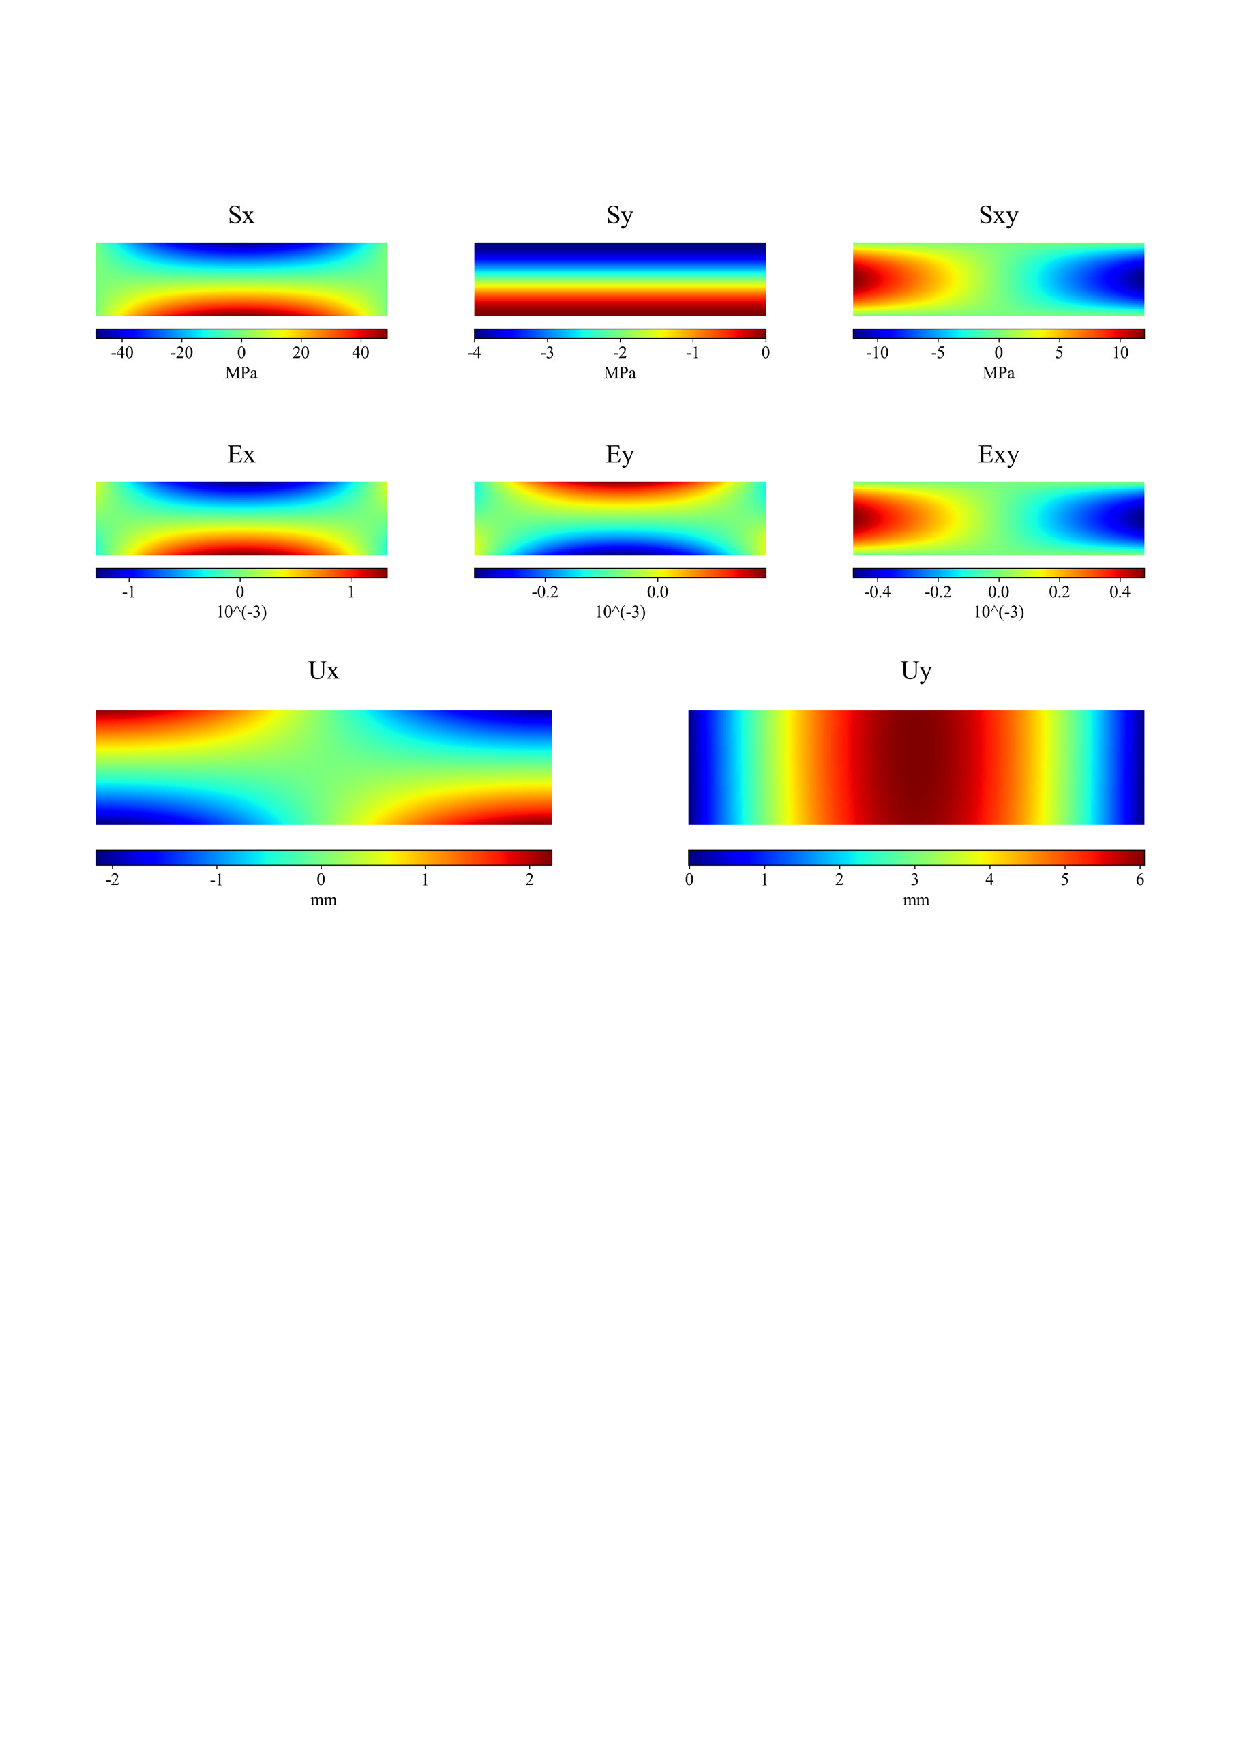
\includegraphics[width=1\textwidth]{figure2}
    \caption{计算结果云图}
    \label{fig:EPMplot}
\end{figure}
\subsection{结果讨论}
本章节,我们将简支梁当作平面应力问题来处理,且假设挤压应力~$\sigma_y$~沿~$x$~方向均匀分布。由于物体厚度方向尺寸较小,且受到的外力和约束只在梁的上下左右四个面,在前后面无约束。所以认为是平面应力问题是精确的。从结果来看,应力分量满足平衡微分方程、相容方程与边界条件,说明对挤压应力~$\sigma_y$~函数形式的假设这种是正确的。两端由于是小边界,即便不严格满足边界条件,对离两边较远处的应力也无影响。

实际问题中,梁厚度方向的尺寸不能满足平面应力问题的条件,且受到的外力和约束会更加复杂。以此为前提,想要得到解析解是十分困难的,因此,借助数值方法对实际问题进行求解得到的结果会对实际工程更有帮助。
\chapter{理想弹塑性材料杆的理论求解}
\label{cha:ideal_theory}
本章节将推导圆杆变形之后,轴向应力与剪应力沿杆截面分布的解析表达式。

首先轴向拉伸细杆,使其全长全截面轴向应力均达到~{$f_y$},建立柱坐标系,此时圆杆内任一横截面上距离轴线~{$x$}距离为~{$r$}的点的应力状态为:
\begin{equation}\label{eq4}
    \sigma_{ij} = \begin{bmatrix}
        0 & 0 & 0 \\
        0 & f_y & 0 \\
        0 & 0 & 0
        \end{bmatrix}
\end{equation} 

偏应力张量:
\begin{equation}\label{eq5}
    s_{ij} = \begin{bmatrix}
        -\frac{1}{3}f_y & 0 & 0 \\
        0 & \frac{2}{3}f_y & 0 \\
        0 & 0 & -\frac{1}{3}f_y
        \end{bmatrix}
\end{equation} 

代入~Mises~屈服准则,求得:
\begin{equation}\label{eq6}
    q = \frac{f_y}{\sqrt{3}}
\end{equation} 

考虑将杆的两个端截面相对旋转一个小角度~{$\theta$},则单位扭转角为:
\begin{equation}\label{eq7}
    \alpha  = \frac{\theta }{L}
\end{equation} 

根据几何关系,柱坐标系下的微应变张量的各分量为:
\begin{equation}\label{eq8}
    \left\{
        \begin{array}{l}
            \varepsilon_rr = \dfrac{\partial u_r}{\partial r}; \varepsilon_{\theta\theta} = \dfrac{\partial u_\theta}{\partial \theta}; \varepsilon_xx = \dfrac{\partial u_x}{\partial x}\vspace{1ex}\\
            \varepsilon_{r\theta} = \dfrac{1}{2}(\dfrac{1}{r}\dfrac{\partial u_r}{\partial \theta}+\dfrac{\partial u_\theta}{\partial r}-\dfrac{u_\theta}{r})\vspace{1ex}\\
            \varepsilon_{\theta x} = \varepsilon_{x \theta}=\dfrac{1}{2}(\dfrac{1}{r}\dfrac{\partial u_x}{\partial \theta}+\dfrac{\partial u_\theta}{\partial x})\vspace{1ex}\\
            \varepsilon_{xr} = \varepsilon_{rx}=\dfrac{1}{2}(\dfrac{\partial u_x}{\partial r}+\dfrac{\partial u_r}{\partial x})\\
        \end{array}
    \right.
\end{equation} 

此时圆杆的位移场:
\begin{equation}\label{eq9}
    \left\{
        \begin{array}{l}
            u_x = \dfrac{f_y}{E}x \vspace{1ex}\\
            u_\theta = axr\\
        \end{array}
    \right.
\end{equation} 

则有:
\begin{equation}\label{eq10}
    \varepsilon_{\theta x} =\dfrac{1}{2}(\dfrac{1}{r}\dfrac{\partial u_x}{\partial \theta}+\dfrac{\partial u_\theta}{\partial x})=\dfrac{1}{2}ar=\dfrac{\theta r}{2L}
\end{equation} 

此时圆杆上各点的应变状态为:
\begin{equation}\label{eq11}
    \varepsilon_{ij} = \begin{bmatrix}
        \varepsilon_{rr} & 0 & 0 \vspace{1ex}\\
        0 & \varepsilon_{xx} & \dfrac{\theta r}{2L} \vspace{1ex}\\
        0 & \dfrac{\theta r}{2L} & \varepsilon_{\theta \theta}
        \end{bmatrix}
\end{equation} 

由问题叙述已知,扭转过程中杆长不变,则~{$\varepsilon_{rr}$}、{$\varepsilon_{xx}$}、~{$\varepsilon_{\theta \theta}$}~在旋转过程中保持不变。因此,可得应变率张量:
\begin{equation}\label{eq12}
    \dot e_{ij} = \dot \varepsilon_{ij} - \dfrac{1}{3}\dot \varepsilon_{ij} \delta_{ij}  = \begin{bmatrix}
        0 & 0 & 0 \vspace{1ex}\\
        0 & 0 & \dfrac{\dot\theta r}{2L}\\
        0 & \dfrac{\dot\theta r}{2L} & 0
        \end{bmatrix}
\end{equation} 

此外,写出此时圆杆各点应力状态:
\begin{equation}\label{eq13}
    \sigma_{ij} = \begin{bmatrix}
        0 & 0 & 0 \\
        0 & \sigma_{xx} & \tau_{x \theta}\\
        0 & \tau_{\theta x} & 0
        \end{bmatrix}
\end{equation} 

则有偏应力张量:
\begin{equation}\label{eq14}
    s_{ij} = \begin{bmatrix}
        -\dfrac{1}{3}\sigma_{xx} & 0 & 0 \vspace{1ex}\\
        0 & \dfrac{2}{3}\sigma_{xx} & \tau_{x \theta}\vspace{1ex}\\
        0 & \tau_{\theta x} & -\dfrac{1}{3}\sigma_{xx}
        \end{bmatrix}
\end{equation} 

相对应的偏应力率张量:
\begin{equation}\label{eq15}
    \dot s_{ij} = \begin{bmatrix}
        -\dfrac{1}{3}\dot \sigma_{xx} & 0 & 0 \vspace{1ex}\\
        0 & \dfrac{2}{3}\dot \sigma_{xx} & \dot \tau_{x \theta}\vspace{1ex}\\
        0 & \dot \tau_{\theta x} & \dfrac{1}{3}\dot \sigma_{xx}
        \end{bmatrix}
\end{equation} 

考虑相关塑性流动法则下,基于~Mises~屈服准则建立的多维弹塑性理论模型。偏应力率与偏应变率的解析求解关系:

因为此时圆杆内各点屈服,由~Mises~屈服函数可得:

整理得圆杆截面各点正应力 与剪应力 满足屈服条件:





\chapter{两种解法的对比分析}
\label{cha:comparison}
\chapter{理想弹塑性材料杆的有限元分析}
\label{cha:abaqus}
本章节使用商业有限元软件~ABAQUS~求解第~\ref{cha:ideal_theory}、第~\ref{cha:hardened}~章对应问题的数值解。自拟了一组参数,比较理论结果与计算结果,讨论二者的区别与联系。
\section{有限元模型的建立}
\subsection{有限元模型参数}
模型建立的基本参数见表~\ref{tab:abaqus}。
\begin{table}[htbp]
    \centering
    \caption{有限元建模参数}\label{tab:abaqus}
    \begin{tabular}{!{\vrule width 1.5pt}c|c|c|c|c|c!{\vrule width 1.5pt}}
    \noalign{\hrule height 1.5pt}
    杆长 & 半径 & 弹性模量 & 泊松比 & 屈服强度 & 扭转角 \\
    \hline
    $250~\text{mm}$ & $10~\text{mm}$ & $2.06\times10^5~\text{MPa}$ & $0.3$ & $235~\text{MPa}$ & $0.1~\text{rad}(5.73^\circ)$ \\
    \noalign{\hrule height 1.5pt}
    \end{tabular}
\end{table}
\subsection{网格划分}
模型采用拉伸实体建模,采用六面体单元、中性轴算法划分网格,模型网格划分情况如图~\ref{fig:mesh}~所示
\begin{figure}[htbp]
    \centering
	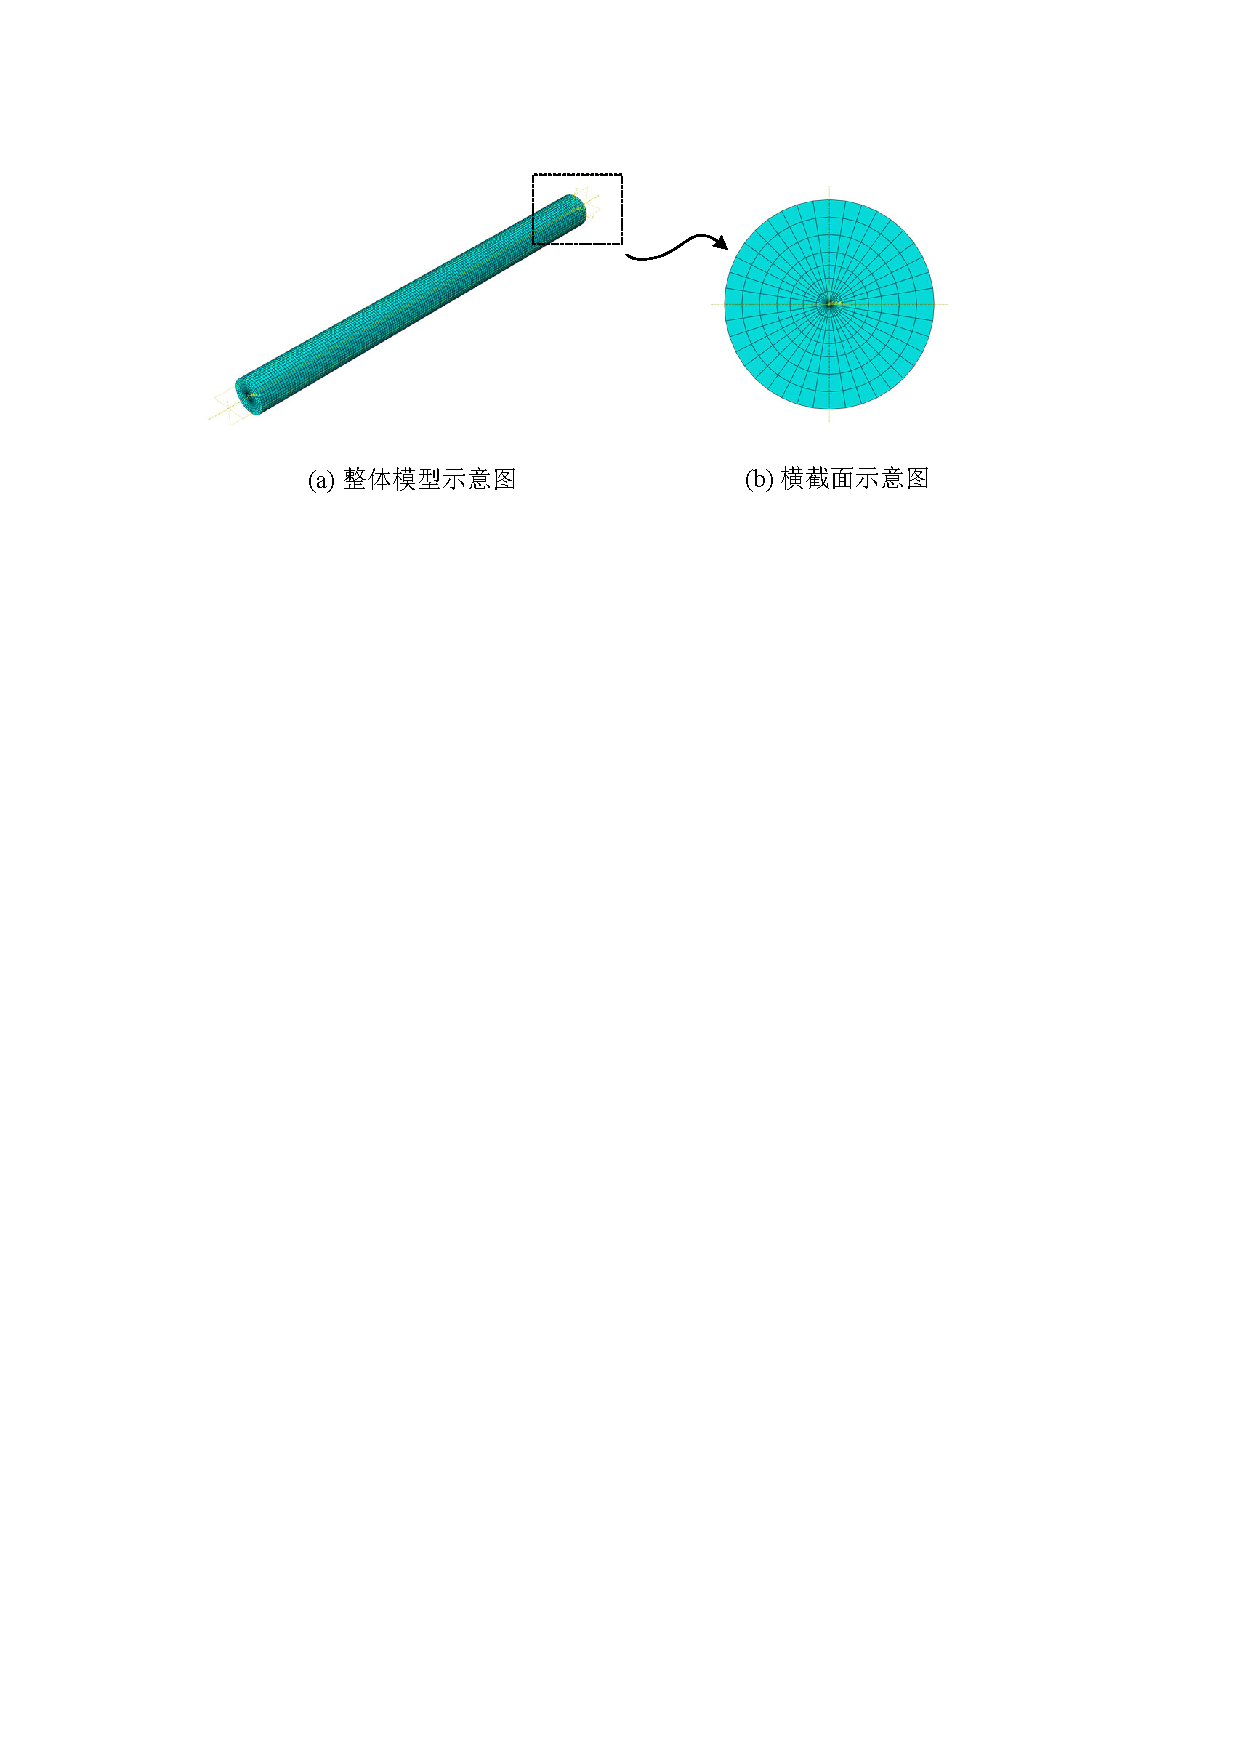
\includegraphics[width=0.7\textwidth]{mesh.pdf}
    \caption{网格划分}
    \label{fig:mesh}
\end{figure}
\subsection{加载过程模拟}
根据题目要求,有限元模型加载过程如下:

(1)在杆两侧截面中心分别设置参考点,并各自与端界面采用~coupling~约束绑定;

(2)分析步~1:将远端参考点完全固定定;

(3)分析步~2:近端参考点设置沿~Z~向的位移,大小为~0.2852~mm,使其全长全截面轴向应力均达到~{$f_y$};

(4)分析步~3:令近端参考点旋转~0.1~rad;

(5)提交作业,进行圆杆全加载过程有限元计算,并对结果进行对比分析。

\section{有限元分析结果}
圆杆~S33(即轴向力)应力云图,S23(即剪应力)应力云图和圆杆跨中截面正应力与剪应力分布云图如图所示如图~\ref{fig:ideal}~所示。
\begin{figure}[htbp]
    \centering
	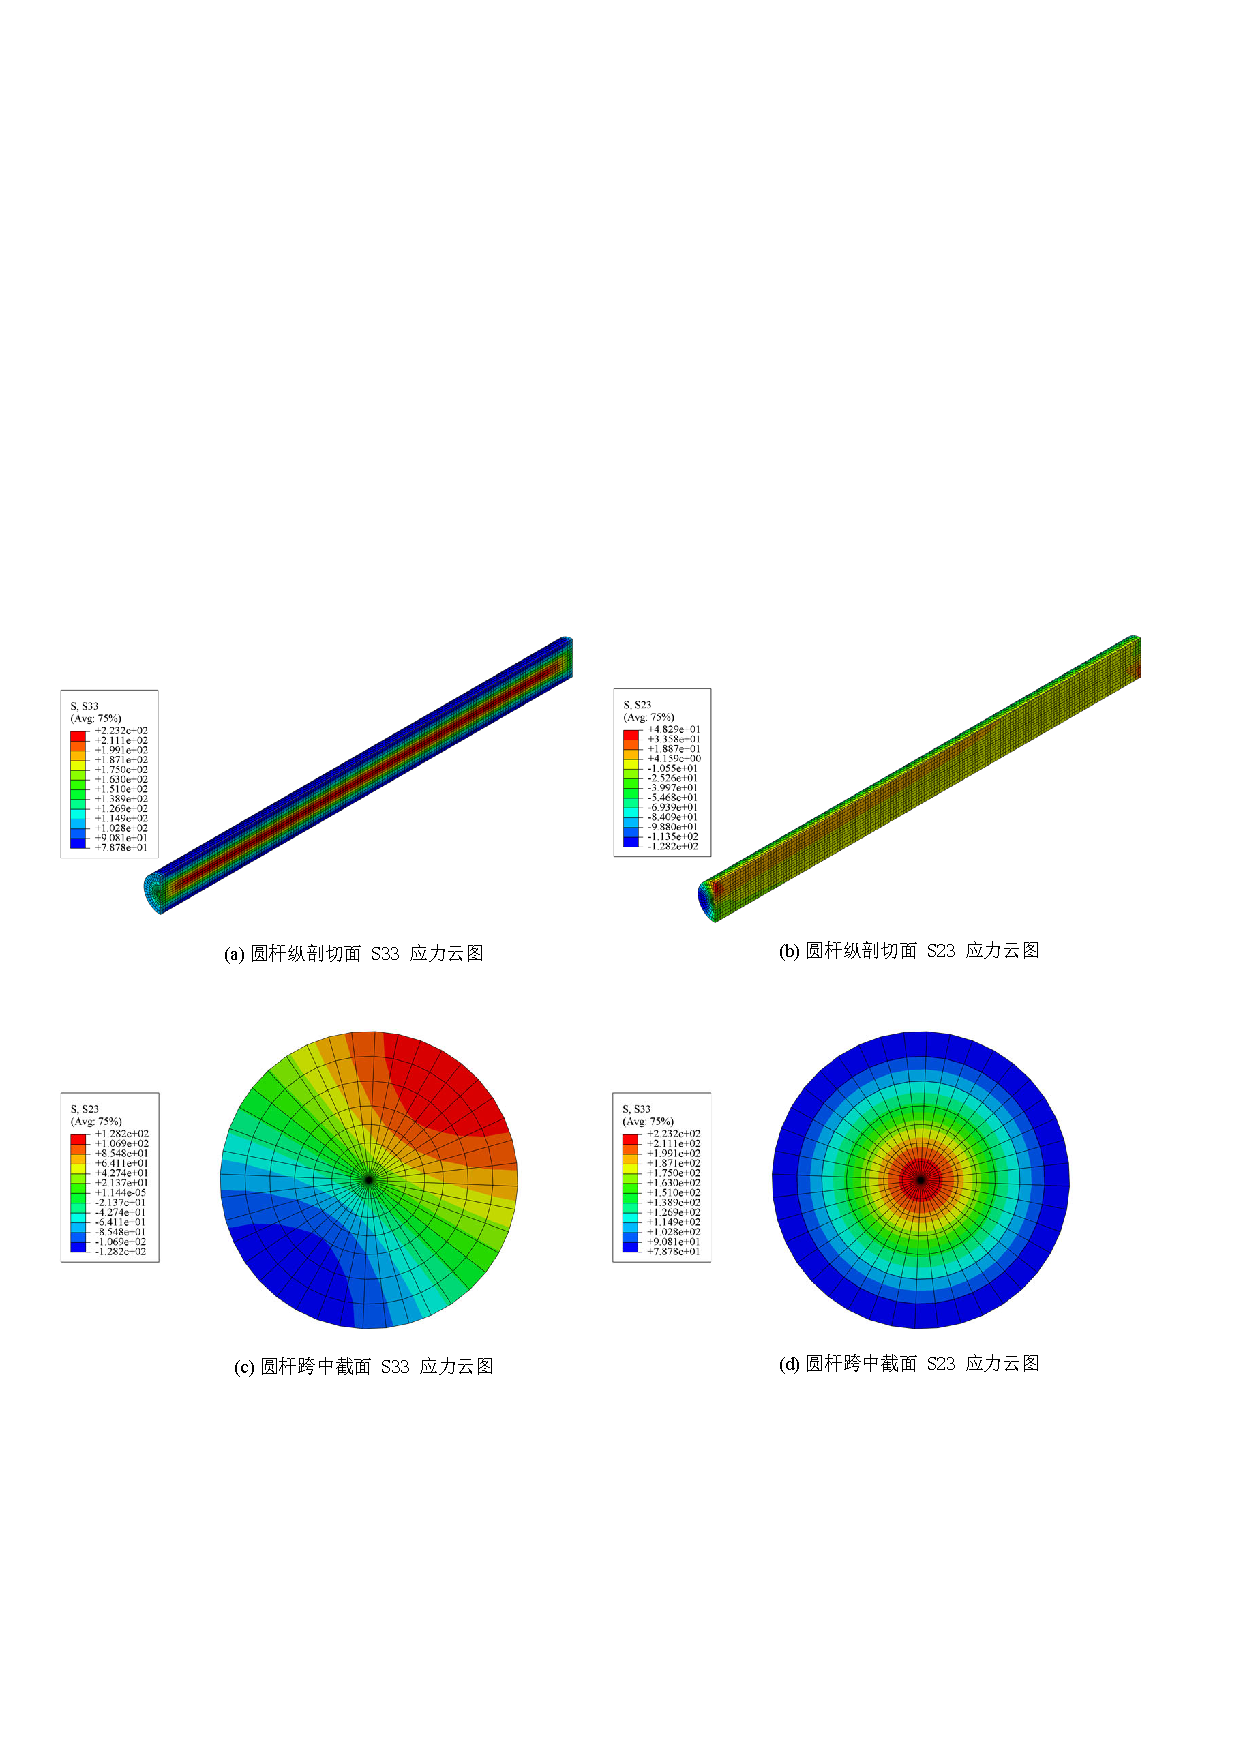
\includegraphics[width=1.0\textwidth]{ideal.pdf}
    \caption{理想弹塑性圆杆数值模拟应力结果}
    \label{fig:ideal}
\end{figure}
\section{有限元分析结果与理论值对比}
导出圆杆跨中截面正应力与剪应力的径向分布结果,并由式~\eqref{eq27}~计算对应的理论值。数值解和解析解的结果如表~\ref{tab:ideals33}、表~\ref{tab:ideals23}~所示,绘制两者对比的散点图如图~\ref{fig:ideals3323}~所示。

由截面正应力与剪应力的纵向分布图、跨中截面正应力与剪应力的径向分布图可知,总体而言理论模型与有限元分析模型较为符合。圆杆跨中截面上各点的正应力随着点到圆心的距离增大而减小,剪应力随着距离的增大而增大,有限元分析结果与理论计算结果趋势一致。
\begin{table}[htbp]
    \centering
    \caption{截面正应力~S33~有限元解与理论解对比}\label{tab:ideals33}
    \begin{tabular}{!{\vrule width 1.5pt}c|c|c|c!{\vrule width 1.5pt}}
    \noalign{\hrule height 1.5pt}
    点到圆心距离($\text{mm}$) & 有限元解($\text{MPa}$) & 理论解($\text{MPa}$) & 相对误差($\text{\%}$) \\
    \hline
    0.00 & 222.22 & 235.00 & 5.44 \\
    \hline
    1.25 & 214.58 & 227.33 & 5.61 \\
    \hline
    2.50 & 194.74 & 206.64 & 5.76 \\
    \hline
    3.75 & 169.34 & 178.38 & 5.07 \\
    \hline
    5.00 & 141.78 & 148.12 & 4.28 \\
    \hline
    6.67 & 114.07 & 111.06 & -2.71 \\
    \hline
    8.33 & 90.22 & 81.02 & -11.35 \\
    \hline
    10.00 & 79.74 & 58.25 & -36.89 \\
    \noalign{\hrule height 1.5pt}
    \end{tabular}
\end{table}
\begin{table}[htbp]
    \centering
    \caption{截面正应力~S23~有限元解与理论解对比}\label{tab:ideals23}
    \begin{tabular}{!{\vrule width 1.5pt}c|c|c|c!{\vrule width 1.5pt}}
    \noalign{\hrule height 1.5pt}
    点到圆心距离($\text{mm}$) & 有限元解($\text{MPa}$) & 理论解($\text{MPa}$) & 相对误差($\text{\%}$) \\
    \hline
    0.00 & 0.00 & 0.00 & 0.00 \\
    \hline
    1.25 & 40.98 & 34.38 & -19.20 \\
    \hline
    2.50 & 69.10 & 64.61 & -6.94 \\
    \hline
    3.75 & 90.99 & 88.33 & -3.01 \\
    \hline
    5.00 & 106.80 & 105.33 & -1.40 \\
    \hline
    6.67 & 118.08 & 119.57 & 1.25 \\
    \hline
    8.33 & 125.10 & 127.36 & 1.77 \\
    \hline
    10.00 & 127.65 & 131.44 & 2.89 \\
    \noalign{\hrule height 1.5pt}
    \end{tabular}
\end{table}

对于截面正应力,在靠近圆心附近,截面正应力的有限元解略小于理论解,相对误差较小,低于~6\% ,而在靠近截面边缘附近,截面正应力的有限元解大于理论解,并且相对误差随着距离的增大而增加,在截面边缘处二者相对误差达到最大,为~36.89\%;对于截面剪应力,在圆心附近,截面剪应力的有限元解大于理论解,且相对误差较大,为~19.2\%,而在靠近截面边缘附近,有限元解略小于理论解,相对误差较小,低于~3\%。

分析误差造成的原因可能有:

(1)有限元模型圆心附近网格划分较为紧密,柱面边缘处的网格划分较为稀疏,可能影响有限元分析结果的准确性。

(2)理论模型的截面应力公式推导仅考虑了剪切应变,并且忽略了材料塑性体积应变,而有限元模型能较为真实的反应圆杆在整个加载过程的应变变化情况,这将造成二者之间有较大误差。

(3)为了更清晰地展示截面应力变化情况,有限元模型在扭转加载阶段选择了较大的扭转角~0.1~rad,这可能导致与理论模型推导过程中的小变形假设不符,造成较大误差。
\begin{figure}[htbp]
    \centering
	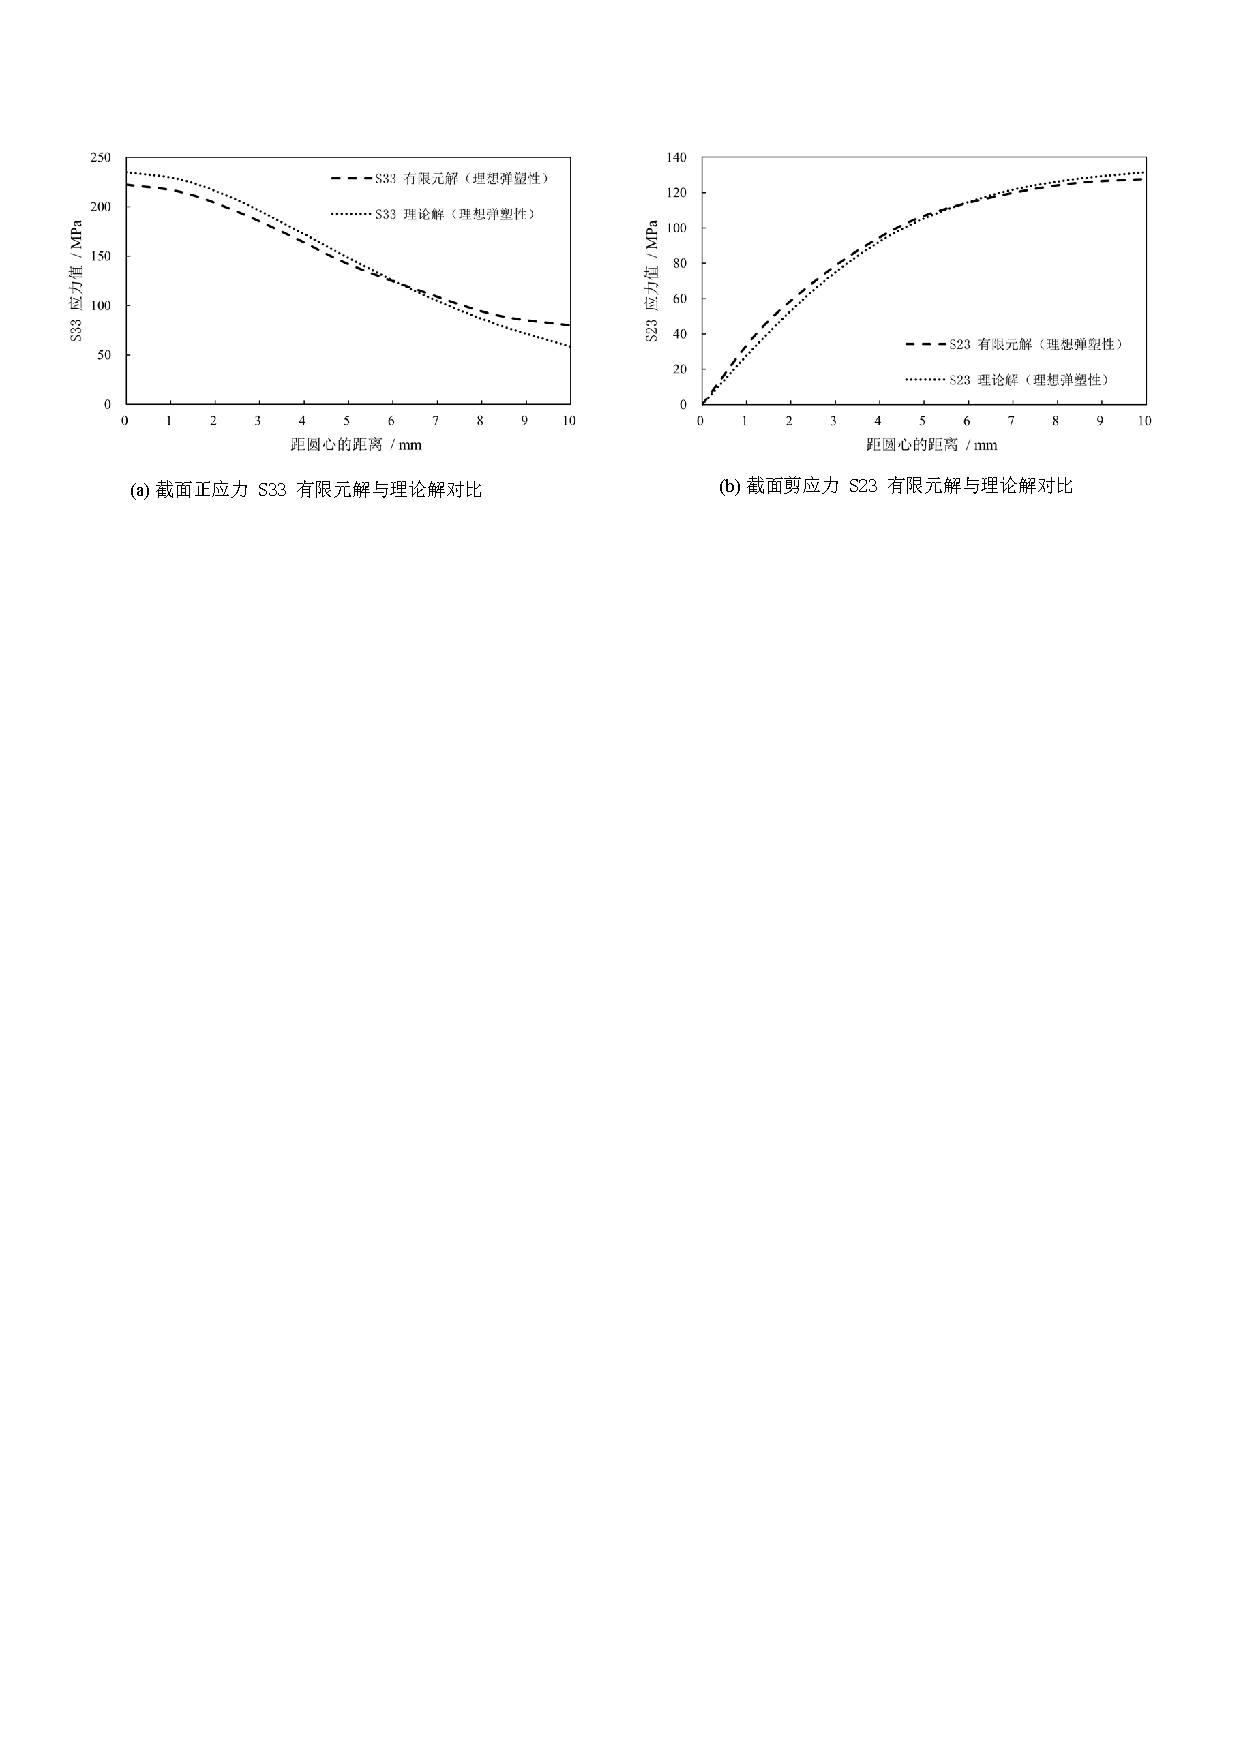
\includegraphics[width=1\textwidth]{1.pdf}
    \caption{理想弹塑性圆杆数值解与解析解对比}
    \label{fig:ideals3323}
\end{figure}







\chapter{各向同性线性硬化材料杆的有限元分析}
\label{cha:abaqus_hardened}

\chapter{D-P~模型材料杆的有限元分析}
\label{cha:abaqus_hardened}

\chapter{总结}
\label{cha:conclusion}

% 致谢
\begin{acknowledgement}
衷心感谢王彦博老师和任晓丹老师在弹塑性力学课程上的悉心教导。两位老师深入浅出的讲解使我对这一复杂的领
域有了更清晰的理解,特别是在如何将理论知识应用于实际工程问题。

在这个课程的学习过程中,我深刻体会到了教学的重要性和学生的学习动力。王老师在课堂上仔细讲解公式的推导,把书本上抽象的数理推演转变为容易让人理解的物理关系。

在课堂上,任老师提到的弹塑性力学与现代科技的交叉应用,尤其是在人工智能领域的潜在发展,
让我倍感振奋。如今~AI~技术在工程设计、材料优化和结构分析等方面的应用日益广泛。我深刻
认识到弹塑性力学的基础知识对于理解和开发这些智能算法,如物理信息系统等是多么重要。
未来,我希望能将所学知识与人工智能相结合,探索如何通过机器学习和数据分析技术,进一
步优化材料性能和结构设计。


再次感谢您为我们付出的努力与心血!
\end{acknowledgement}

% 附录
\begin{appendix}
    \chapter{外部资料声明}
\label{cha:statement}
本文使用的~\LaTeX{}~模板,解析解云图绘制代码,有限元分析云图等文件均已上传至作者的~GitHub,可以在~\url{https://github.com/Charlie-is-charlie/BEPmechanics}~中查看并下载。
\end{appendix}

% 参考文献
\printTJbibliography

\end{document}
